\chapter{Elvégzett munka}


\section{Koncepció}
Állapottérképek formális verifikációjának támogatása MagicDraw-ban, egy plug-in fejlesztésével lett megvalósítva. A plug-in függ a Viatra For MagicDraw-tól, ami lehetővé teszi modellek transzformációját, ennek a felhasználásával a plug-n MagicDraw modelleket Gamma modellekké alakít, majd a Gamma egyes részeinek felhasználásával (\ref{fig:used-gamma} ábra) ezeken végrehajtja a formális verifikációt. A plug-in MagicDrawToGammának lett elnevezve.

\begin{figure}[!ht]
	\centering
	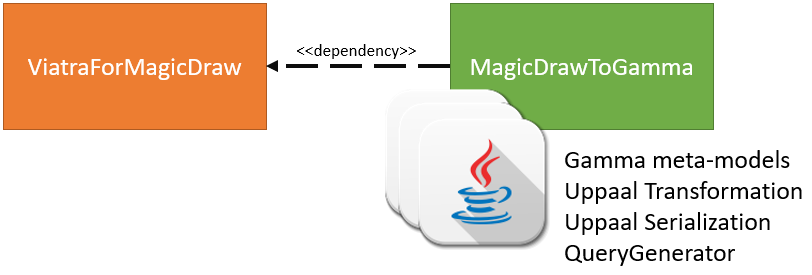
\includegraphics[keepaspectratio, width=120mm]{figures/plan.png}
	\caption{Architektúra koncepció}
	\label{fig:used-gamma}
\end{figure}

\section{Fejlesztés menete}
 A fejlesztés fejlesztő környezet előkészítésével kezdődött. MagicDraw biztosít egy ún. skeletont Eclipsehez és IntelliJhez is plug-in fejlesztéséhez, de a fejlesztés nem ezek segítségével hanem az IncQueryLabs által készített skeleton felhasználásával valósult meg. Ez már elő volt készítve V4MD használatához.
 
A skeleton Eclipsehez készült, viszont Gradlet használ a projekt fordításához és a dependenciák kezeléséhez. A következő lépés ezek meghatározása volt.

\subsection{Gamma függőségek}
